\documentclass[10pt]{article}  

%%%%%%%% PREÁMBULO %%%%%%%%%%%%
\title{Tratamiento de datos sobre el dataset del beisbol en USA}
\usepackage[spanish]{babel} %Indica que escribiermos en español
\usepackage[utf8]{inputenc} %Indica qué codificación se está usando ISO-8859-1(latin1)  o utf8  
\usepackage{amsmath} % Comandos extras para matemáticas (cajas para ecuaciones,
% etc)
\usepackage{amssymb} % Simbolos matematicos (por lo tanto)
\usepackage{color}
\usepackage{graphicx}
\usepackage{epsfig}
\usepackage{multirow}
\usepackage{colortbl}
\usepackage{graphicx} % Incluir imágenes en LaTeX
\usepackage{color} % Para colorear texto
\usepackage{booktabs} % 
\usepackage[utf8]{inputenc} % Permite usar acentos
\usepackage{subfigure} % subfiguras
\usepackage{float} %Podemos usar el especificador [H] en las figuras para que se
% queden donde queramos
\usepackage{capt-of} % Permite usar etiquetas fuera de elementos flotantes
% (etiquetas de figuras)
\usepackage{sidecap} % Para poner el texto de las imágenes al lado
	\sidecaptionvpos{figure}{c} % Para que el texto se alinie al centro vertical
\usepackage{caption} % Para poder quitar numeracion de figuras
\usepackage{commath} % funcionalidades extras para diferenciales, integrales,
% etc (\od, \dif, etc)
\usepackage{cancel} % para cancelar expresiones (\cancelto{0}{x})
 
\usepackage{anysize} 					% Para personalizar el ancho de  los márgenes
\marginsize{2cm}{2cm}{2cm}{2cm} % Izquierda, derecha, arriba, abajo

\usepackage{appendix}
\renewcommand{\appendixname}{Apéndices}
\renewcommand{\appendixtocname}{Apéndices}
\renewcommand{\appendixpagename}{Apéndices} 

% Para que las referencias sean hipervínculos a las figuras o ecuaciones y
% aparezcan en color
\usepackage[colorlinks=true,plainpages=true,citecolor=blue,linkcolor=blue]{hyperref}
%\usepackage{hyperref} 
% Para agregar encabezado y pie de página
\usepackage{fancyhdr} 
\pagestyle{fancy}
\fancyhf{}
\fancyhead[L]{\footnotesize TRATAMIENTO INTELIGENTE DE DATOS} %encabezado izquierda
\fancyhead[R]{\footnotesize }   % dereecha
\fancyfoot[R]{\footnotesize }  % Pie derecha
\fancyfoot[C]{\thepage}  % centro
\fancyfoot[L]{\footnotesize Master en Ingeniería Informática}  %izquierda
\renewcommand{\footrulewidth}{0.4pt}

\definecolor{lightgray}{gray}{0.9}

\usepackage{listings} % Para usar código fuente
\definecolor{dkgreen}{rgb}{0,0.6,0} % Definimos colores para usar en el código
\definecolor{gray}{rgb}{0.5,0.5,0.5} 
% configuración para el lenguaje que queramos utilizar
\lstset{language=Matlab,
   keywords={break,case,catch,continue,else,elseif,end,for,function,
      global,if,otherwise,persistent,return,switch,try,while},
   basicstyle=\ttfamily,
   keywordstyle=\color{blue},
   commentstyle=\color{red},
   stringstyle=\color{dkgreen},
   numbers=left,
   numberstyle=\tiny\color{gray},
   stepnumber=1,
   numbersep=10pt,
   backgroundcolor=\color{white},
   tabsize=4,
   showspaces=false,
   showstringspaces=false}

\newcommand{\sen}{\operatorname{\sen}}	% Definimos el comando \sen para el seno
%en español

\title{Dataset de la liga de beisbol en USA}

%%%%%%%% TERMINA PREÁMBULO %%%%%%%%%%%%

\begin{document}

%%%%%%%%%%%%%%%%%%%%%%%%%%%%%%%%%% PORTADA %%%%%%%%%%%%%%%%%%%%%%%%%%%%%%%%%%%%%%%%%%%%
																					%%%
\begin{center}																		%%%
\newcommand{\HRule}{\rule{\linewidth}{0.5mm}}									%%%\left
 																					%%%
\begin{minipage}{0.48\textwidth} \begin{flushleft}

\includegraphics[scale = 0.35]{Imagenes/logougr.eps}
\end{flushleft}\end{minipage}
\begin{minipage}{0.48\textwidth} \begin{flushright}

\includegraphics[scale = 0.63]{Imagenes/decsailogo.eps}
\end{flushright}\end{minipage}

													 								%%%
\vspace*{0.5cm}								%%%
																					%%%	
\textsc{\huge Universisdad de Granada}\\[1.5cm]	

%\textsc{\LARGE Unidad Profesional Interdisciplinaria en Ingenier\'ia y				%%%
%Tecnolog\'ias Avanzadas}\\[1.5cm]													%%%

\begin{minipage}{0.9\textwidth} 
\begin{center}																					%%%
\textsc{\LARGE Aplicación de la minería de datos}
\end{center}
\end{minipage}\\[0.5cm]
%%%
    																				%%%
 			\vspace*{1cm}																		%%%
																					%%%
\HRule \\[0.4cm]																	%%%
{ \huge \bfseries Tratamiento de Datos sobre el dataset del beisbol en USA}\\[0.4cm]	%%%
 																					%%%
\HRule \\[1.5cm]																	%%%
 																				%%%
																					%%%
\begin{minipage}{0.46\textwidth}													%%%
\begin{flushleft} \large															%%%
\emph{Autores:}\\	
Manuel Jesús García Manday
\\Mario Ortega Aguayo
%%%
			%\vspace*{2cm}	
            													%%%
										 						%%%
\end{flushleft}																		%%%
\end{minipage}		
																%%%
\begin{minipage}{0.52\textwidth}		
\vspace{-0.6cm}											%%%
\begin{flushright} \large															%%%
													%%%
\end{flushright}																	%%%
\end{minipage}	
\vspace*{1cm}
%\begin{flushleft}
 	
%\end{flushleft}
%%%
 		\flushleft{\textbf{\Large Master en  Ingeniería Informática}	}\\																		%%%
\vspace{2cm} 																				
\begin{center}																					
{\large \today}																	%%%
 			\end{center}												  						
\end{center}							 											
																					
\newpage																		
%%%%%%%%%%%%%%%%%%%% TERMINA PORTADA %%%%%%%%%%%%%%%%%%%%%%%%%%%%%%%%

\tableofcontents 

\newpage


\section{Introducción} 

A través de la minería de datos es posible extraer información relevante sobre conjuntos grandes de datos aplicando una serie de técnicas y algoritmos que se encargan de explorarlos.\\


En este documento se mostrará la exploración de un conjunto de datos utilizando para ello algunas de las técnicas mas comunes como la clasificación, la regresión y el agrupamiento, exponiendo en cada punto del presente trabajo el tratamiento aplicado así como la interpretación de los resultados. \\

Son varias las herramientas existentes para explorar grandes conjuntos de datos, Knime y R Studio son de las más comunes y utilizadas en este ámbito. En esta ocasión he decidido trabajar con R Studio por ser una herramienta basada en scripts de R y tener algo de experiencia previa, lo que me ayudará a incrementarla y profundizar en su conocimiento. \\

\section{Dataset} 

Tras investigar y navegar por diferentes sitios web como kaggle.com que ofrecen múltiples datasets , hemos optado por seleccionar un conjunto de datos aplicado al ámbito del deporte. En este caso el baseball, un deporte mundialmente conocido y que tiene su principal foco en los Estados Unidos desde hace muchos años.\\

Hemos seleccionado este dataset después de analizarlo y evaluar las diferentes variables y observaciones que presenta, viendo que sería interesante conocer y profundizar más sobre los detalles de este deporte. \\

Este conjunto de datos contiene información completa de los equipos de baseball de la liga de los Estados Unidos desde 1871 hasta 2015, en dichos datos se pueden ver estadísticas sobre los bateadores y pitchers de los equipos así como estadísticas los partidos jugados, los partidos ganados y perdidos, los entrenadores, las ligas, etc.  La última versión de este dataset, la cual es la que hemos utilizado, se puede encontrar en la página www.seanlahman.com/baseball-archive, así como versiones anteriores y diferentes formatos del conjunto de datos.\\

Son muchas las variables de las que dispone este dataset, por lo que después de realizar un análisis sobre cada una de ellas viendo lo que puede aportar en el estudio y la relevancia de sus datos, hemos seleccionado un subconjunto de ellas creando un nuevo dataset sobre el que realizaremos todas las técnicas de minería de datos mencionadas anteriormente, manteniendo las mismas filas que en el original.\\


Para evitar que no se seleccionen variables relevanes para el nuevo dataset, hemos realizado un estudio previo de todo el conjunto de variables para eliminar las que tengas valores nulos o que no aporten nada al estudio.  Para ello hemos realizado un análisis exploratorio previo donde poder ver las relaciones entre las diferentes variables del conjunto inicial.\\


Como se puede observar en la siguiente imagen, existen campos en el dataset que no son tan importantes para el estudio como los dos que se han comparado más abajo. En este caso las variables de "media de partidos ganados" y de "factor de 3 años para los bateadores" no van a aportar ninguna conclusión ni dato de peso en el estudio, por lo que estas dos son entre otras más las que no entraran en el conjunto final del dataset.

\begin{figure}[H]
	\begin{center}
 		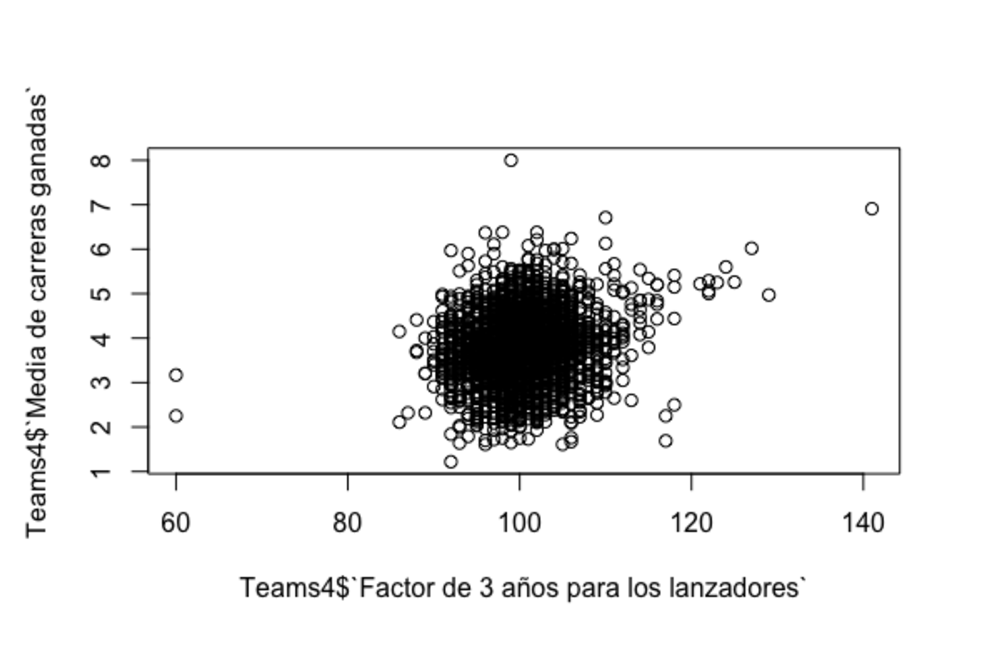
\includegraphics[width = 0.75\textwidth]{Imagenes/preprocesamiento.eps}
 		\captionof{figure}{\label{fig:IPN}} 
	\end{center} 
\end{figure}

En la siguiente tabla se muestra un resumen de las variables que representan este nuevo conjunto de datos en función a cada equipo que ha participado en la liga de baseball entre los años 1871 y 2015, indicando su tipo y medida:\\


\begin{table}[htbp]
\begin{center}
\begin{tabular}{|l|l||l|}
\hline
Variable & Tipo  & Medida \\
\hline \hline \hline
yearID & fecha  & año de fundación \\ \hline
lgID & texto  & liga a la que pertenece \\ \hline
Games & número (entero) & partidos jugados \\ \hline
Win & número (entero) & partidos ganados \\ \hline
Lost & número (entero) & partidos perdidos \\ \hline
LgWin & booleano & si ha ganado la liga \\ \hline
R & número (entero) & carreras anotadas \\ \hline
AB & número (entero) & veces que un bateador cambia contra un pitcher \\ \hline
H & número (entero) & golpes de los bateadores \\ \hline
SO & número (entero) & strikeouts de los bateadores \\ \hline
SB & número (entero) & bases robadas \\ \hline
RA & número (entero) & carreras anotadas por el contrario \\ \hline
CG & número (entero) & juegos completados \\ \hline
SHO & número (entero) & juego terminado en el que el equipo perdedor no anota carrera \\ \hline
E & número (entero) & errores \\ \hline
\end{tabular}
\caption{Conjunto de varibales.}
\label{Tabla:}
\end{center}
\end{table}

Como se ha podido comprobar en la anterior tabla, el conjunto de datos seleccionado contiene información sobre los aspectos meramente deportivos sucedidos durante el transcurso de todos los partidos disputados por cada equipo en el periodo indicado anteriormente, de la cual se puede obtener conclusiones curiosas e importantes como veremos en los posteriores puntos de este trabajo.

	

\section{Análisis exploratorio}

Una vez que se ha dispuesto del nuevo dataset con el subconjunto de variables del original y manteniendo el mismo número de datos (mismo número de fila), hemos realizado un primer análisis exploratorio sobre las diferentes variables para comenzar a ver la relación que existe entre los diferentes campos y obtener resultados que nos ayude mejor a comprender este conjunto de datos.\\

\begin{figure}[H]
	\begin{center}
 		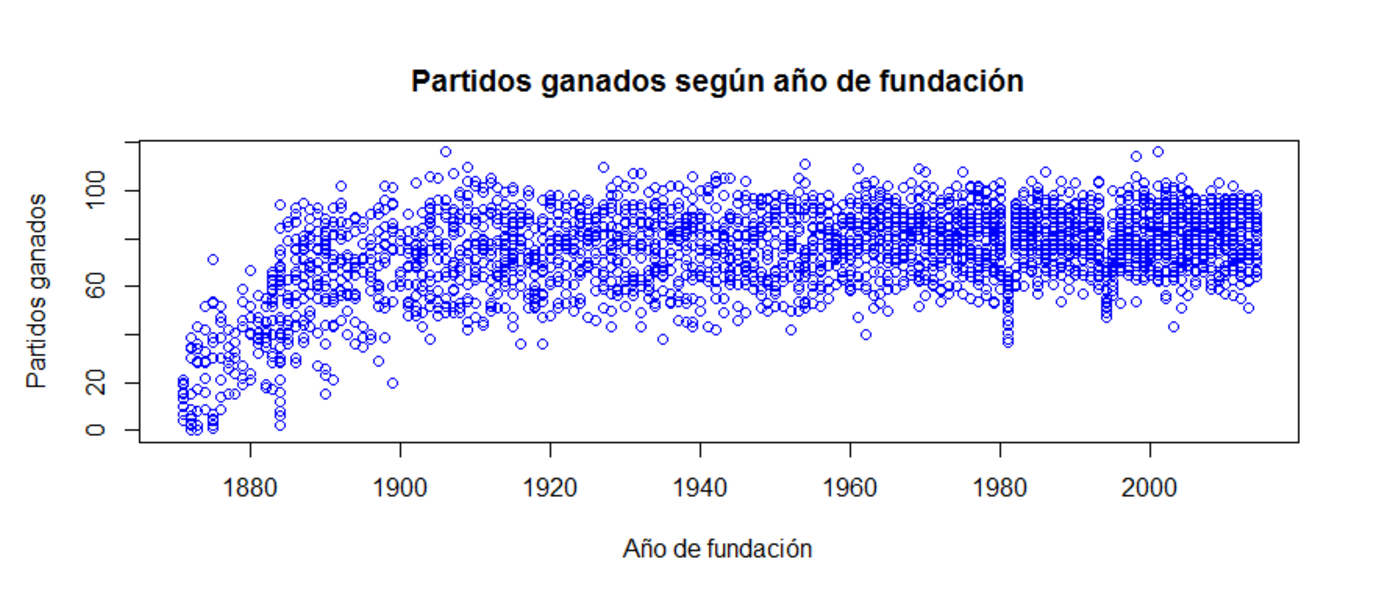
\includegraphics[width = 0.75\textwidth]{Imagenes/prepocesamiento1.eps}
 		\captionof{figure}{\label{fig:IPN}} 
	\end{center} 
\end{figure}

En este primer análisis realizado sobre el conjunto de datos podemos ver como el número de partidos ganados tiene un crecimiento a finales del siglo XIX y principios del siglo XX, esto puede ser debido a que la cantidad de equipos y partidos aumentaran durante esa época. Lo que también se puede observar es durante el periodo de finales del siglo XX y comienzos del siglo XXI son más la cantidad de puntos sobre la gráfica, lo que no interviene en la cantidad de partidos ganados ya que se mantiene en la misma línea, sino que refleja el crecimiento en número de equipos durante ese periodo, que fue la época dorada del baseball en los Estados Unidos según su historia.\\

\begin{figure}[H]
	\begin{center}
 		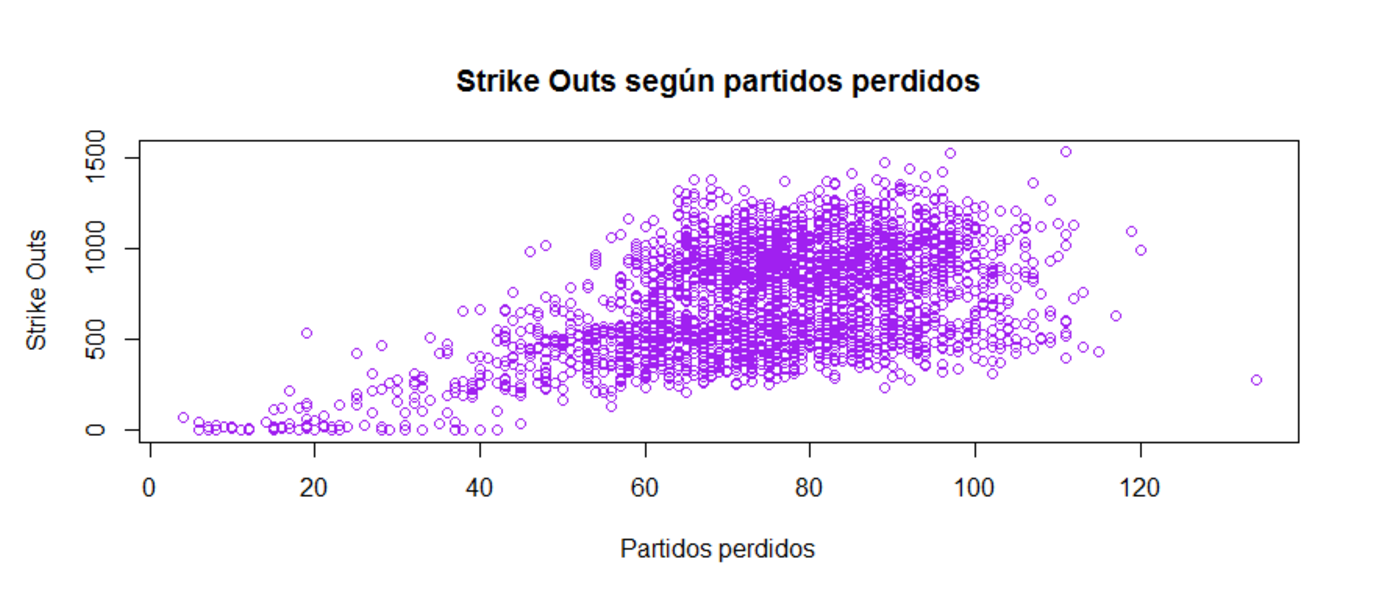
\includegraphics[width = 0.75\textwidth]{Imagenes/preprocesamiento2.eps}
 		\captionof{figure}{\label{fig:IPN}} 
	\end{center} 
\end{figure}

La Figura 3 muestra la relación existente entre el número de partidos perdidos y la cantidad de strikes outs acumulados. Como se puede observar los resultados obtenidos son totalmente razonables y casan con la lógica, ya que la mayor cantidad de strikes outs se encuentran concentrados en el rango de mayor número de partidos perdidos que va de 60 a 100. Esto se debe a que en un partido de baseball, un strike out penaliza al equipo que lo comete, ya que elimina a uno de sus bateadores. \\

\begin{figure}[H]
	\begin{center}
 		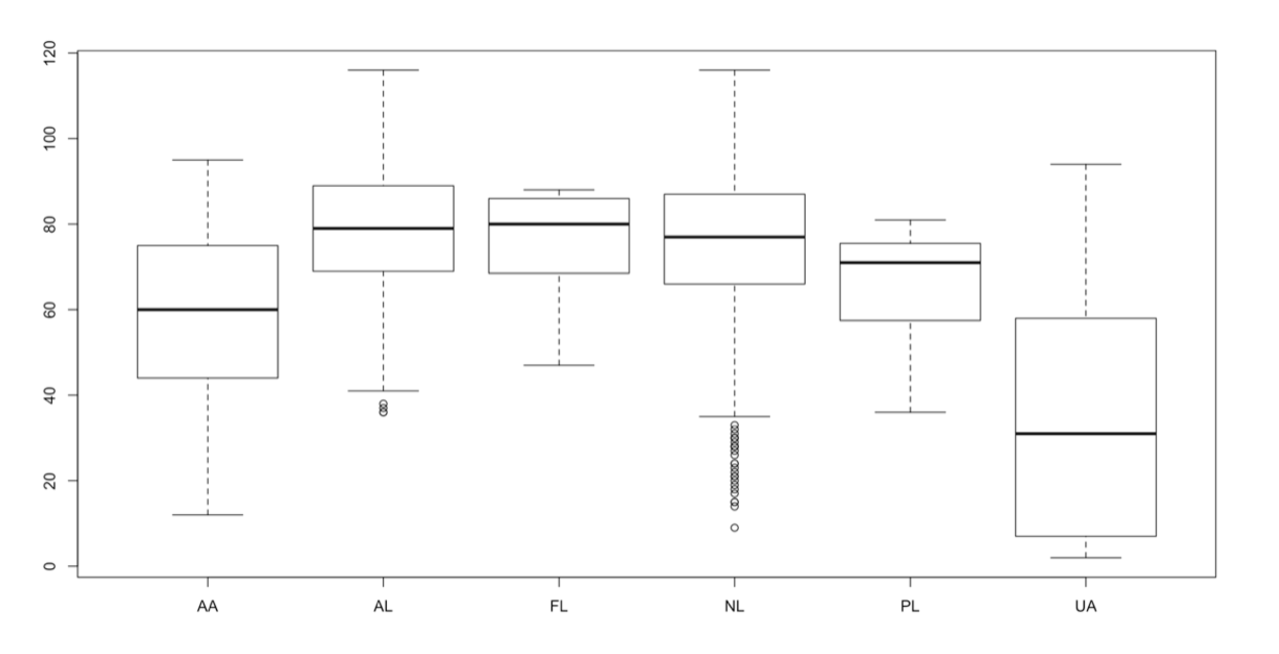
\includegraphics[width = 0.75\textwidth]{Imagenes/prepocesamiento3.eps}
 		\captionof{figure}{\label{fig:IPN}} 
	\end{center} 
\end{figure}

Para la Figura 4 se ha utilizado otro tipo de gráfico para expresar la relación entre la cantidad de partidos ganados y la liga en los que se han disputados. Observando la gráfica anterior se puede como existen 3 ligas que son las que mayor número de victorias han conseguido sus equipos, siendo la liga UA la que menor puntuación tiene. Esto puede ser debido a la calidad de los diferentes equipos en relación a sus jugadores, algo que si duda afecta en el ámbito de cualquier deporte. Otro detalle a tener en cuenta que arroja esta gráfica es la disposición de la raya horizontal negra dentro de cada caja (lo que es conocido como bigote), que como podemos observar en dos de ellas no se encuentra situadas en la mitad de la misma, sino que la separación entre la parte superior y la parte inferior que divide dicha raya horizontal es diferente, esto es debido a que la cantidad de partidos ganados en esas ligas fueron conseguidos por un número menor de equipos, es decir, el número de victorias en esas ligas estás concentradas en un menor número de equipos que en las demás ligas.



\section{Clustering}

Cuando tenemos un dataset con una cantidad elevada de datos, estos se muestran aparentemente complicados de organizar.\\

La técnica clustering consiste en clasificar los datos formando grupos o clusters de elementos, de forma que los datos dentro de cada agrupacion presenten cierto grado de homogeneidad en base a los valores adoptados sobre un conjunto de variables. Para 
nuestro dataset, vamos a utilizar el algoritmo kmeans de R para realizar el cluster.\\

Una vez que se han eliminado los datos vacíos dentro de nuestro dataset a analizar, se cogen variables que aparentemente tengan relación, asi podremos ver mejor la bondad de esta técnica. Cabe destacar que se han seleccionado para este nuevo conjunto variables que no tienen mucha relación entre ellas para ver como se comporta la bondad en este caso. \\

De esta manera podremos aplicar la técnica de clustering a variables que tienen una mayor bondad frente a otras que tienen menos y poder sacar conclusiones referente a las agrupaciones obtenidas.\\

En la siguiente tabla se muestran los campos que se han escogido del dataset con el hemos comenzado el estudio de tratamiento de datos:\\

\begin{table}[htbp]
\begin{center}
\begin{tabular}{|l|l|}
\hline
Variable & Medida \\
\hline \hline
yearID & año de fundación  \\ \hline
Games & partidos jugados \\ \hline
AB & veces que un bateador cambia contra un pitcher \\ \hline
SHO & juego terminado en el que el equipo perdedor no anota carrera \\ \hline
SB & bases robadas \\hline
E & errores \\ \hline
\end{tabular}
\caption{Conjunto de varibales para Clustering.}
\label{Tabla:}
\end{center}
\end{table}

Una vez con el subconjunto seleccionado, procedemos a estandarizar las variables y así tener las mismas unidades, es decir, una desviación estándar.\\

Kmeans es un algoritmo de partición de datasets en distintos grupos, donde se clasifican según similitudes que hay entre ellos. 
Hemos decidido utilizar este algoritmo ya que consideramos que es más idóneo para analizar un gran número de casos, y por otro lado no es necesario trabajar sobre una matriz distancias, sino que la hace sobre la original, y así no requiere tanto uso de procesamiento y consumo de memoria. \\

El algoritmo va asignando a un grupo u otro según el intervalo al que pertenezca. El número de grupos lo determinamos por el valor k, el cual estableceremos en la propia función de R.\\

El primer paso es determinar el número de clústers en que se va a dividir el conjunto sobre el que se va a trabajar, cuestión que no es fácil de determinar. Sin embargo, usa solución usada frecuentemente para determinar el número óptimo de clusters es el método Elbow (del inglés codo, referente a la curvatura que se forma en la gráfica), el cual implica observar un conjunto de posibles números de agrupaciones en relación con la forma en que minimizan la suma de cuadrados dentro del grupo. Vemos la gráfica a continuación y observamos como el número óptimo de clusters sería 4, ya que es el punto en que tiende a decrementar.\\

\begin{figure}[H]
	\begin{center}
 		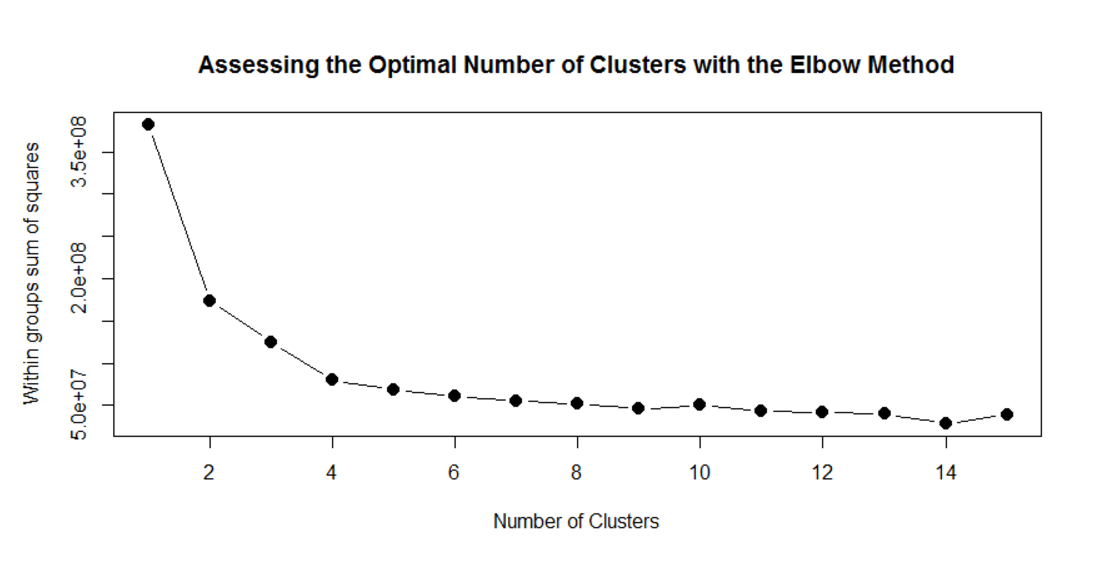
\includegraphics[width = 0.75\textwidth]{Imagenes/numcluster.eps}
 		\captionof{figure}{\label{fig:IPN}} 
	\end{center} 
\end{figure}

Para comprobar este hecho, en primer lugar vamos a hacer un clustering con 2 y 3 grupos, como vemos a continuación.\\


\begin{figure}[H]
	\begin{center}
 		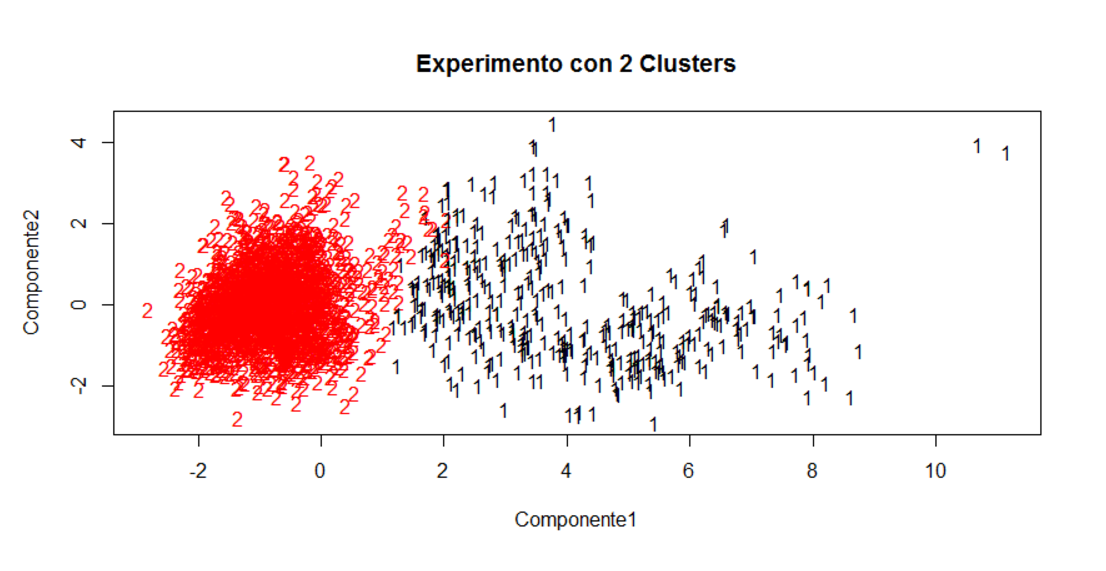
\includegraphics[width = 0.75\textwidth]{Imagenes/2clusters.eps}
 		\captionof{figure}{\label{fig:IPN}} 
	\end{center} 
\end{figure}


\begin{figure}[H]
	\begin{center}
 		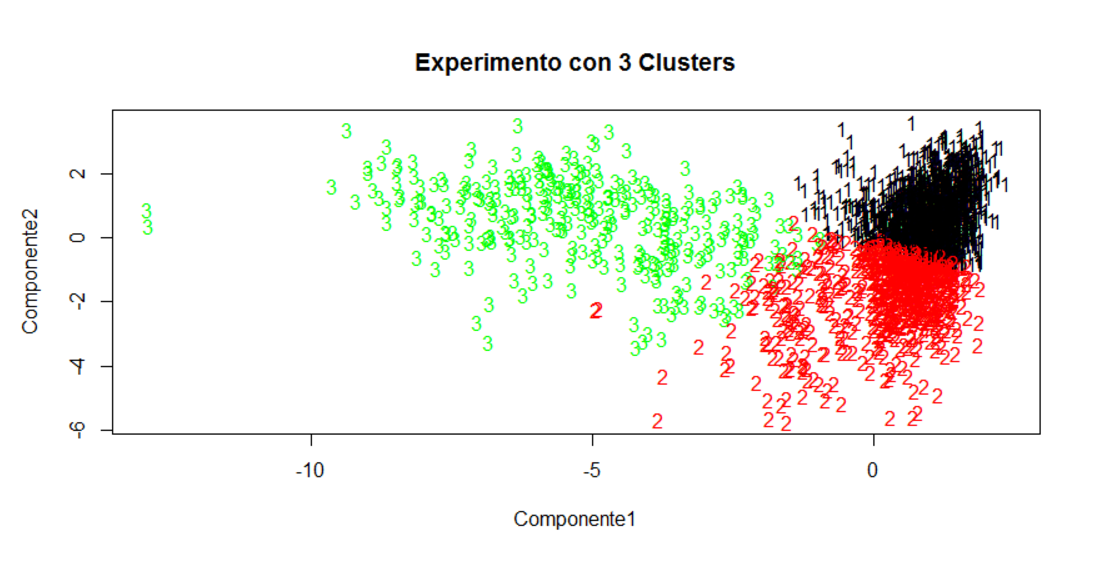
\includegraphics[width = 0.75\textwidth]{Imagenes/3clusters.eps}
 		\captionof{figure}{\label{fig:IPN}} 
	\end{center} 
\end{figure}

Como observamos, en la solución para 2 clusters se crean dos conjuntos diferenciados pero uno de ellos es bastante disperso, por lo que no podremos concluir que haya muchas similitudes entre los conjuntos.\\

En la solución para 3 clusters se crean igualmente dos grupos que parecen tener bastante similitud pero uno disperso y no demasiado mezclado con los grupos restantes.\\

A continuación vamos a ver la restante, con 4 clusters, como ya comentamos anteriormente sería el más óptimo para este conjunto de datos.\\

\begin{figure}[H]
	\begin{center}
 		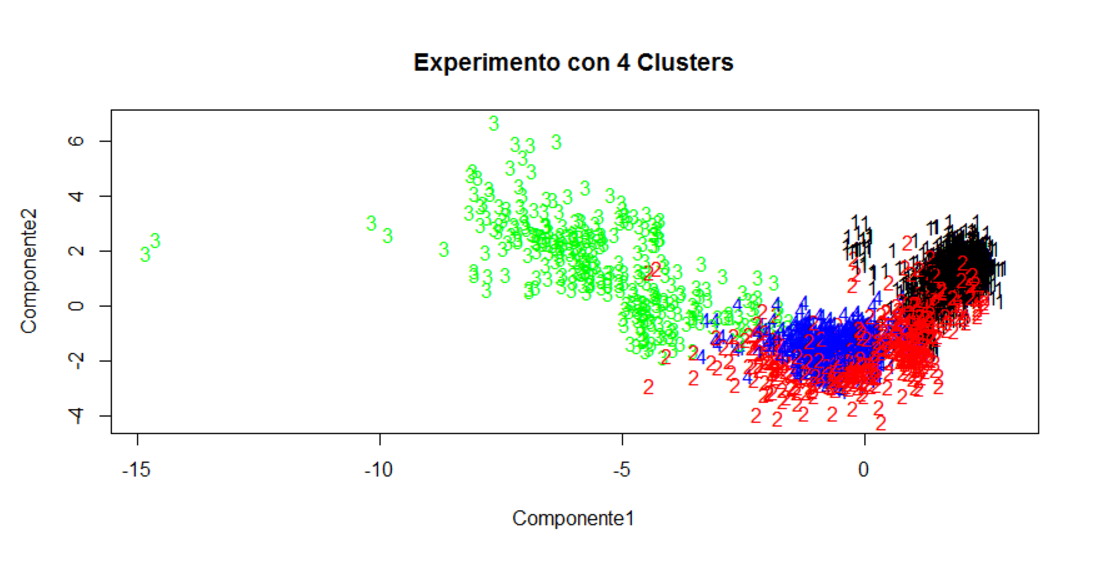
\includegraphics[width = 0.75\textwidth]{Imagenes/4clusters.eps}
 		\captionof{figure}{\label{fig:IPN}} 
	\end{center} 
\end{figure}

Como podemos ver en la gráfica, a pesar de que un conjunto se mantiene disperso, los 3 conjuntos restantes estan bastante mezclados y cercanos, por lo que entre ellos se observa bastante similitud.


\section{Árboles de decisión}

Mediante los árboles de decisión vamos a clasificar en diversos grupos los equipos para de este modo predecir si un equipo puede ganar la liga o no en función de los valores de las variables del modelo. Con el conjunto de datos ya cargado, lo siguiente es cargar una serie de librerías necesarias para trabajar con los árboles de decisión, en este caso utilizaremos la librería rpart. \\

\textbf{library(rpart)} \\
\textbf{library(rpart.plot)} \\

Ahora vamos a generar dos conjuntos más de manera aleatoria, uno para entrenamiento y otro para los test. \\

\textbf{indice = sample(2, row(Teams2), replace=TRUE, prob=c(0.7, 0.3))} \\
\textbf{entrenaTeams = Teams2[indice==1,]} \\
\textbf{testTeams = Teams2[indice==2,]}\\

Una vez generado los dos conjuntos de muestreo con la probabilidad indicada en el parámetro correspondiente, lo siguiente será describir el modelo de clasificación, junto con la clase y las variables que intervienen, y crear el árbol de decisión, así como la predicción.\\

\textbf{modeloTeams = LgWin ~ R + H + SO + RA}
\textbf{arbolTeams = rpart(modeloTeams, data=entrenaTeams)}
\textbf{arbolTeams2 = rpart(modeloTeams, data=entrenaTeams, parms=list(split="information"))}

\textbf{plot(arbolTeams)}
\textbf{text(arbolTeams)}
\textbf{plot(arbolTeams2)}
text(arbolTeams2)

\textbf{prediccion = predict(myModel, testTeams)}
\textbf{mc = table(prediccion, entrenaTeams.LgWin)}

\textbf{rpart.plot(arbolTeams, type=1, extra=100, cex=.7, box.col=c("gray99", "gray88")[arbolTeams.LgWin])}\\

El árbol de decisión obtenido al realizar la clasificación con dicho modelo es el que se muestra en las figuras de abajo.

\begin{figure}[H]
	\begin{center}
 		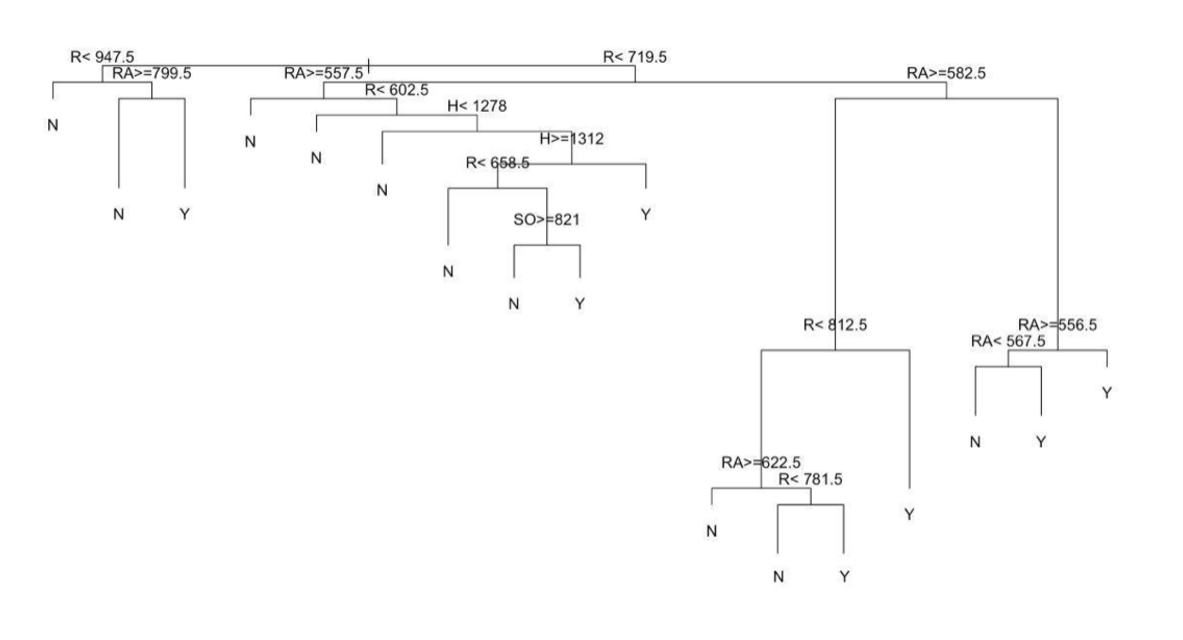
\includegraphics[width = 0.75\textwidth]{Imagenes/arbol1.eps}
 		\captionof{figure}{\label{fig:IPN}} 
	\end{center} 
\end{figure}

\begin{figure}[H]
	\begin{center}
 		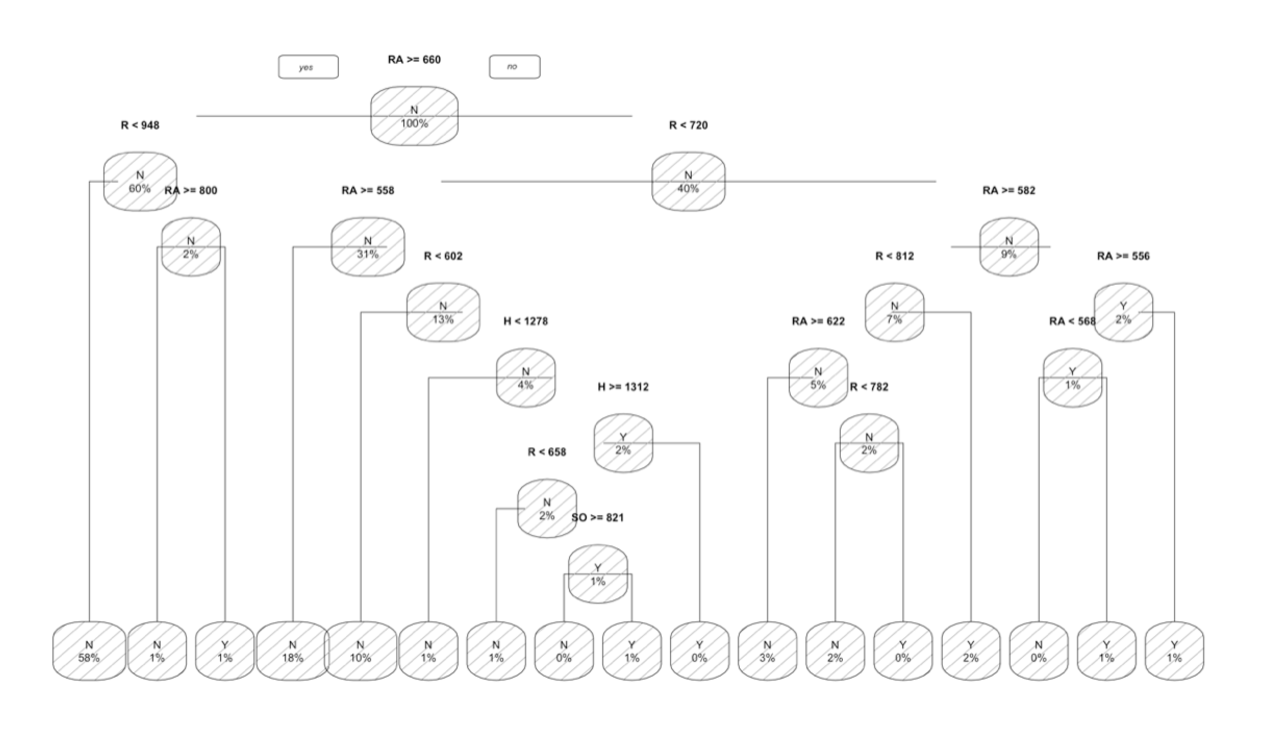
\includegraphics[width = 0.95\textwidth]{Imagenes/arbol2.eps}
 		\captionof{figure}{\label{fig:IPN}} 
	\end{center} 
\end{figure}

\begin{figure}[H]
	\begin{center}
 		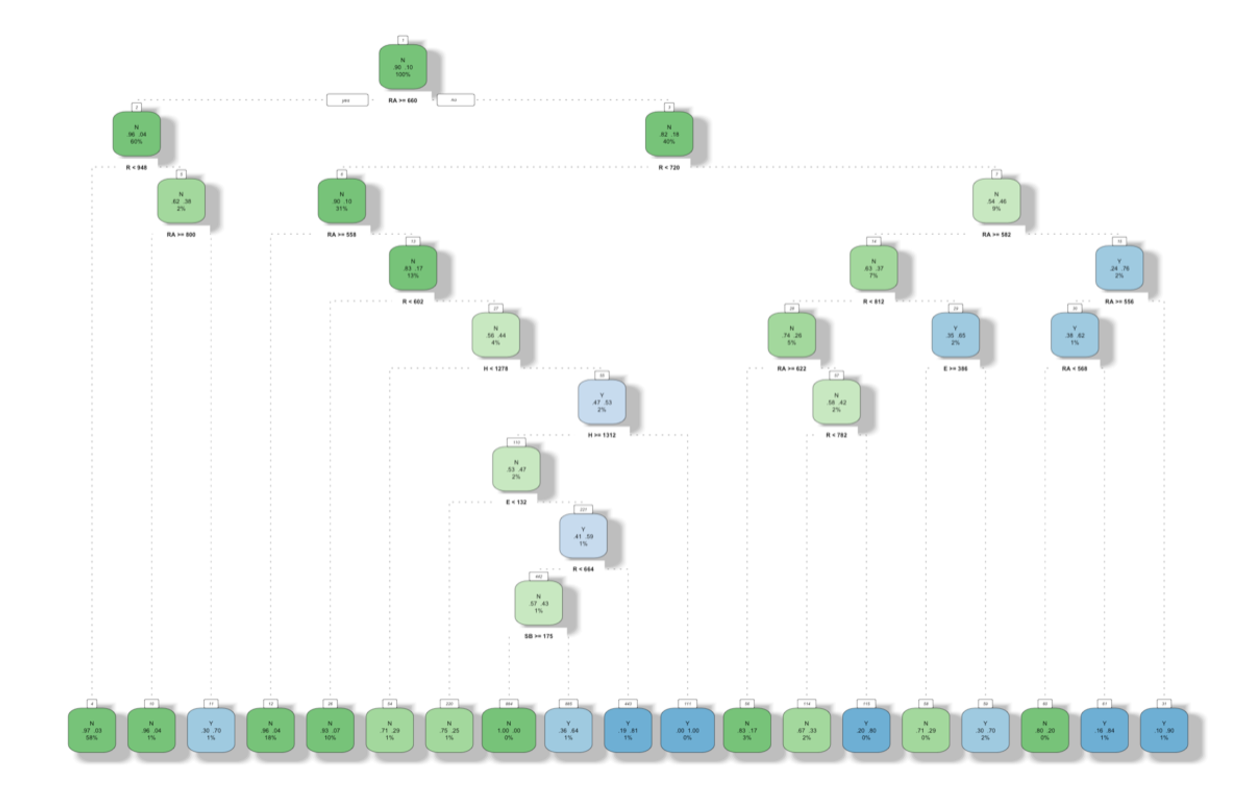
\includegraphics[width = 0.95\textwidth]{Imagenes/arbol3.eps}
 		\captionof{figure}{\label{fig:IPN}} 
	\end{center} 
\end{figure}

Como se ha podido comprobar en las imágenes anteriores, la clasificación se ha realizado en base a todas las variables del modelo, lo cual quiere decir que el modelo utilizado mantiene una buena relación entre todas ellas. Observando los resultados obtenidos vemos que el porcentaje de ganar la liga en función de esas variables es muy bajo, debido a que son muchas las observaciones sobre las que se ha realizado (más de 2700 equipos) y que sólo hay un campeón por año en cada liga, por lo que la predicción para ganar una liga determinada en función de los resultados que obtenga el equipo en base a las variables del modelo es bajo como los que muestran en las Figuras 9, 10 y 11.\\


\section{Regresión}

Para la realización del método de regresión lineal se van a comparar los siguientes campos:\\

\begin{table}[htbp]
\begin{center}
\begin{tabular}{|l|l|}
\hline
Variable & Medida \\
\hline \hline
W & total de partidos ganados \\ \hline
H & golpes de los bateadores \\ \hline
R & carreras anotadas \\ \hline
\end{tabular}
\caption{Conjunto de varibales para Regresión.}
\label{Tabla:}
\end{center}
\end{table}

Como podemos imaginar, son campos que pueden tener una alta relación. En primer lugar, se ejecuta el método pairs, el cual nos va a relacionar pares de gráficos de dispersión y encontramos la siguiente imagen.\\

En una primera visualización, podemos observar que el campo H y R, en especial, van a tener una relación positiva, aunque en las otras comparaciones también encontraremos una buena relación.\\

\begin{figure}[H]
	\begin{center}
 		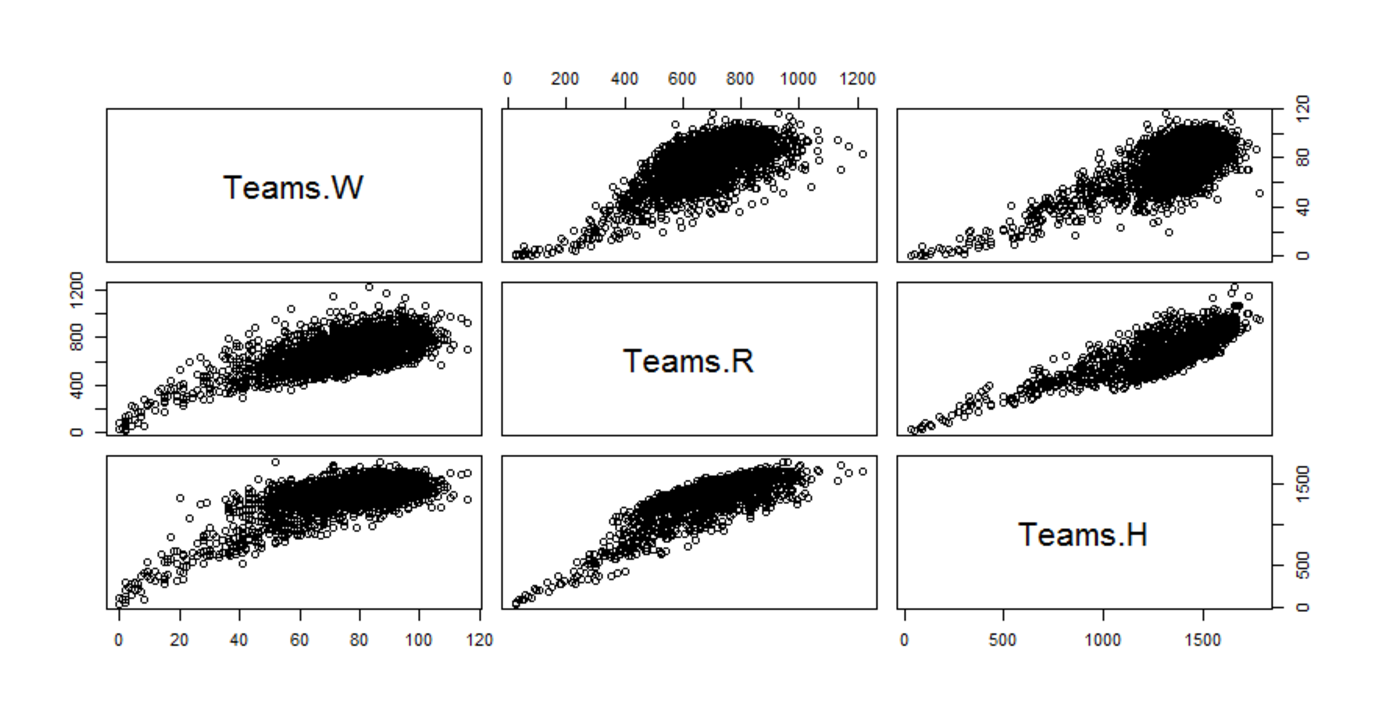
\includegraphics[width = 0.95\textwidth]{Imagenes/regresion.eps}
 		\captionof{figure}{\label{fig:IPN}} 
	\end{center} 
\end{figure}

A continuación se va a ejecutar el método cor, y así visualizaremos una matriz que va a determinar la correlación lineal entre los campos a comparar. Este método nos muestra la siguiente matriz:\\

\begin{table}[htb]
\centering
\begin{tabular}{|l|l|l|l|}
\hline
\cline{2-4}
& Teams.W & Teams.R & Teams.H\\
\hline \hline
{Teams.W} & 1.0000000 & 0.6782768 & 0.7264355\\ \cline{1-4}
{Teams.R} & 0.6782768 & 1.0000000 & 0.8023696\\ \cline{1-4}
{Teams.H} & 0.7264355 & 0.8023696 & 1.0000000\\ \cline{1-4}
\end{tabular}
\label{tabla:final}
\end{table}

Como vemos, R y H tienen una correlación positiva de 80% y H con W de 72%
aproximadamente. Por tanto, son buenos datos para realizar este experimento. Vamos a realizar el experimento sobre las variables de mayor correlación, es decir, los golpes de los
bateadores y las carreras anotadas.\\

Tras esto, creamos un modelo donde relacionamos valores dependientes entre ellos, donde decimos que H (golpes de los bateadores) es dependiente de R (carreras anotadas), siendo H la variable independiente y R la dependiente.\\

Ahora se crea un vector con el comando lineal mode, donde definimos la ecuación, introduciendo en el vector regresión los valores del modelo lineal, a través de los parámetros modelo y el propio dataset.\\

Hacemos un summary para mostrar todas las características de la regresión que acabamos de hacer.\\

\textbf{Call:}\\
\textbf{lm(formula = modelo, data = newteams2)}\\

\textbf{Residuals:}\\
        \textbf{Min       1Q    Median    3Q     Max}\\
     \textbf{-554.47 -44.02   30.90    85.55  271.61}\\

\textbf{Coefficients:}\\
                     \textbf{Estimate      Std. Error t value     Pr(>|t|)}\\
\textbf{(Intercept)   459.10554     12.77059 35.95     <2e-16 ***}\\
\textbf{Teams.R      1.30016          0.01837 70.80     <2e-16 ***}\\

\textbf{Signif. codes: 0 ‘***’ 0.001 ‘**’ 0.01 ‘*’ 0.05 ‘.’ 0.1 ‘ ’ 1}\\

\textbf{Residual standard error: 131.9 on 2773 degrees of freedom}\\
\textbf{Multiple R-squared: 0.6438, Adjusted R-squared: 0.6437}\\
\textbf{F-statistic: 5012 on 1 and 2773 DF, p-value: < 2.2e-16}\\

Vemos que la variable R e Intercepto son significativos a mas del 99 por ciento, ya que lo indica ***. Por tanto, ahora nos aseguramos que podemos crear la gráfica de regresión, a la cual añadiremos la línea que indica que la regresión lineal es creciente y significativa.\\

\begin{figure}[H]
	\begin{center}
 		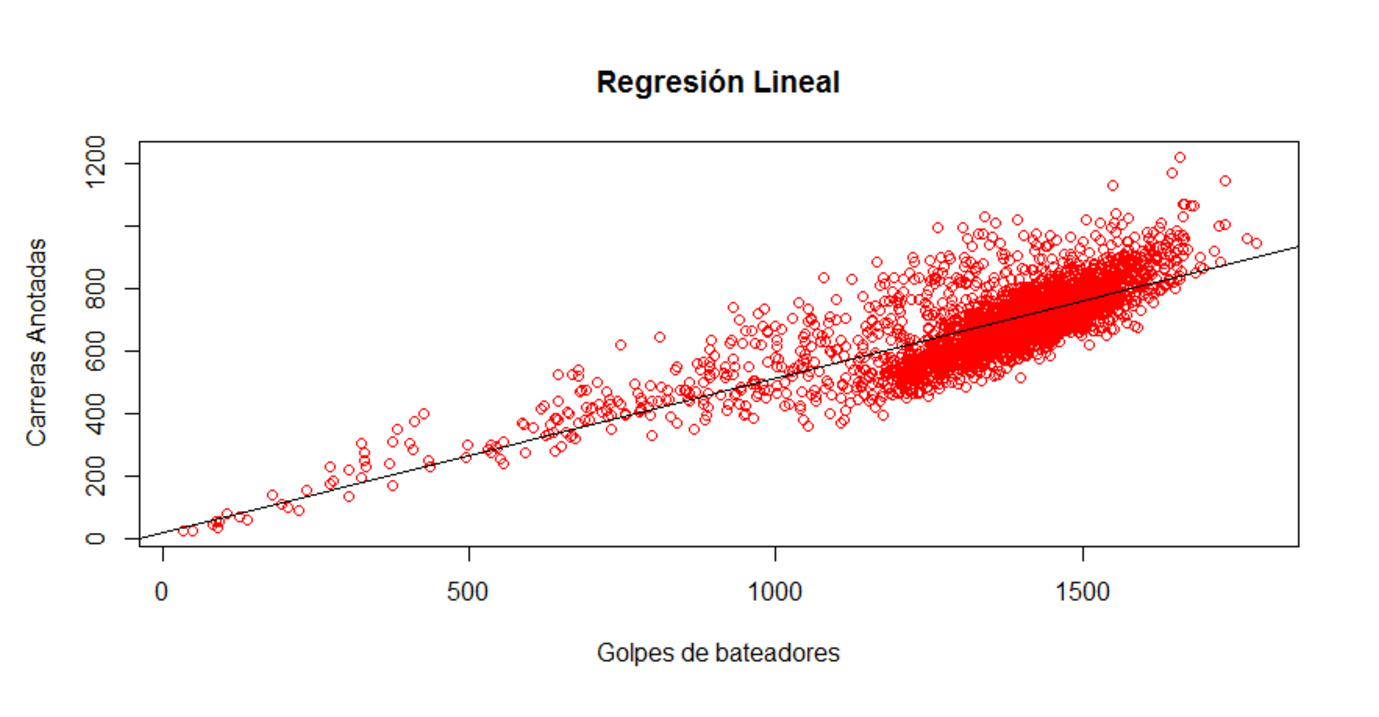
\includegraphics[width = 0.95\textwidth]{Imagenes/regresion1.eps}
 		\captionof{figure}{\label{fig:IPN}} 
	\end{center} 
\end{figure}

Vemos a través de la gráfica de la Figura 13 que es una relación con pendiente positiva, por tanto el experimento ha resultado satisfactorio.\\


\section{Conclusiones}

Hemos decido utilizar un dataset bastante extenso ya que, pensamos que a la hora de llevar este trabajo a un ambiente laboral, la cantidad de datos va a ser bastante grande, por tanto, hemos querido experimentar el abordaje de este tipo de tarea.  Por otro lado, hemos decidido utilizar R, ya que, aparte de tener motivación para aprenderlo, ya que nunca antes habíamos trabajado con el, es un lenguaje robusto, potente y muy utilizado en data mining, por tanto hay un gran volumen de documentación referente al mismo. \\

El análisis de este dataset nos ha permitido profundizar en las técnicas de agrupamiento, clasificación y regresión para grandes volúmenes de datos, mediante los cuales hemos podido sacar importantes deducciones y detalles significativos como pueden ser los factores que se tienen que dar para que un equipo pueda ganar la liga, que la mayoría de los partidos ganados en algunas ligas se concentran en un subconjunto más pequeño de equipos o que existen un incremento positivo en el número de carreras anotadas en función de los golpes certeros de los bateadores.\\

Las técnicas empleadas en este trabajo pensamos que han sido las más adecuadas ya que, como comentamos anteriormente, el dataset tiene un gran volumen. Por ello, pensamos que a través de estos métodos veremos con más claridad el análisis de los datos y obtendremos estadísticas más fiables y más optimas para este tipo de análisis.\\

%%%%%%% Bibliografía %%%%%%%%
\begin{thebibliography}{a}
\bibitem{pradery} \textsc{Dataset.},
\textit{http://www.seanlahman.com/baseball-archive/statistics/}
\bibitem{old} \textsc{Apuntes asignatura Master en Ingeniería Informática},
\textit{https://decsai.ugr.es/}
\end{thebibliography}




\end{document}